% CVPR 2025-based 4+1 research paper (4 content pages + 1 references page).
% Final version: rounds 1-3 and the pre-registered follow-up. Every number is taken from
% paper/inputs/results.json (checked by scripts/check_numbers.py); every citation from inputs/refs.bib.
\documentclass[10pt,twocolumn,letterpaper]{article}
\usepackage{cvpr}
%
% --- inline annotations
%
\newcommand{\red}[1]{{\color{red}#1}}
\newcommand{\todo}[1]{{\color{red}#1}}
\newcommand{\TODO}[1]{\textbf{\color{red}[TODO: #1]}}
% --- disable by uncommenting  
% \renewcommand{\TODO}[1]{}
% \renewcommand{\todo}[1]{#1}


\usepackage{amsmath,booktabs}


\definecolor{cvprblue}{rgb}{0.21,0.49,0.74}
\usepackage[pagebackref,breaklinks,colorlinks,allcolors=cvprblue]{hyperref}
\def\paperID{00000000}
\def\confName{Anonymous Review}
\def\confYear{2026}

\title{Image Labels Are Nearly Enough: A Pre-Registered Study of\\Weakly Supervised Localisation for Zero-Shot Medical Anomaly Detection}
\author{Vismay Shanbhag \quad Dhananjay Bhattacharya \quad Sashakt Keshri\\Kevalina Bhattacharyya \quad Divyam Agarwal\\Birla Institute of Technology and Science, Pilani, K K Birla Goa Campus, Goa, India}

\begin{document}
\maketitle
\begin{abstract}
Pixel masks are the costliest annotation in medical imaging, yet MVFA, a CLIP-based zero-shot medical anomaly detector, learns to localise only from pixel masks, which BMAD provides for only three of its six datasets. We ask how far image-level labels go. Under leave-one-modality-out evaluation on BMAD, with source-only checkpoint selection and decision rules frozen before every round, we tested candidate refinements of image-label training over three rounds and a follow-up. Plain top-$k$ multiple-instance learning (MIL) on image labels alone retains 0.969 of a re-trained MVFA's pixel-AUROC margin over chance (at least 0.924 on every target); two earlier, weaker tests point the same way. With masks for only 10\% of the abnormal source images and image labels elsewhere, localisation on unseen brain MRI exceeds full-mask MVFA on 5/5 pre-registered seeds (mean AUPRO $+14.70$), though not on liver CT. The two refinements we implemented (ranks 1 and 3 of five) did not help, and two earlier apparent gains did not survive replication. Our runs use a reduced training budget, and target image-level AUROC remains weak under source-only selection.
\end{abstract}

\section{Introduction}
\label{sec:intro}
Vision-language models such as CLIP~\cite{clip2021} enable zero-shot anomaly detection, and MVFA adapts CLIP to medical images with residual adapters at four feature levels, trained on five BMAD datasets and tested on an unseen sixth~\cite{huang2024mvfa,bmad2024}. Its segmentation adapters, the only part that draws anomaly maps, are trained with Dice and Focal losses on pixel masks, which exist for only three of the six datasets (brain MRI, liver CT, retinal OCT from RESC). The other three sources (OCT17, chest X-ray, histopathology) carry image labels but never teach localisation. An analysis of MVFA's limitations, checked against its code, points to this dependence on expensive masks. This led to our question: \emph{can MVFA's localisation be learned from image labels, and how much of mask-supervised localisation survives on an unseen modality?}

We answer it with a three-round study in which candidate refinements were ranked in advance and implemented one round at a time, and every claim was decided by rules frozen before the runs. Our contributions are:
\begin{itemize}
\item \textbf{Image labels nearly match masks.} Plain top-$k$ MIL without any mask retains 0.969 of a re-trained MVFA's pixel-AUROC margin (at least 0.924 per target), confirmed under a pre-registered rule in round 3. Rounds 1 and 2 point the same way but were weaker tests (0.966 against the released checkpoint with one seed; 0.930).
\item \textbf{On brain MRI, a small mask budget beats full masks.} With masks for 10\% of the abnormal source images and MIL elsewhere, AUPRO exceeds full-mask MVFA on 5/5 fresh, pre-registered seeds (72.08 vs 57.38). It trails on liver CT and does not improve image-level AUROC.
\item \textbf{A replication record and an audit.} The two refinements we implemented (ranks 1 and 3 of five) failed, and two positives from earlier rounds did not replicate with longer training on fresh seeds. We also found 11 BMAD validation images that duplicate test images (10 of them brain abnormal; we removed them from source validation, so target scores are unaffected), and that MVFA's released training script selects checkpoints on the target test set.
\end{itemize}

\section{Related Work}
\label{sec:related}
\textbf{Vision-language anomaly detection.} CLIP-based detectors such as WinCLIP, APRIL-GAN, AnomalyCLIP, AdaCLIP and VCP-CLIP adapt visual-language features to anomaly detection~\cite{winclip2023,aprilgan2023,anomalyclip2023,adaclip2024,vcpclip2024}. Medical variants, including MediCLIP, IQE-CLIP and MADPOT, target clinical images~\cite{mediclip2024,iqeclip2026,madpot2026}, and BMAD standardises medical anomaly benchmarks across modalities~\cite{bmad2024,medicalad_survey2021}. MVFA~\cite{huang2024mvfa} is our base model; we study only its supervision, not a new architecture.

\textbf{Weak and mask-free localisation.} Multiple-instance learning treats an image as a bag of patches with a bag-level label~\cite{ilse2018attentionmil}. Image-level supervision for anomaly segmentation has been explored through cycle-consistent segmentation, top-$k$ feature adaptation and reasoning-driven localisation~\cite{cycle_seg2021,adfa2023,imagelevel2026}. Memory banks of normal patch features~\cite{patchcore2021} underlie the gated selection we test. AUPRO follows MVTec AD~\cite{mvtec2019}. Other works use different protocols, so we do not compare their numbers.

\textbf{Positive-unlabelled learning.} With normal patches as labelled data and abnormal-image patches as unlabelled mixtures, localisation becomes PU learning~\cite{elkan2008pu}. nnPU keeps the estimated negative risk non-negative~\cite{kiryo2017nnpu}, and mixture-proportion estimation recovers the class prior only under irreducibility~\cite{ramaswamy2016mpe}.

\section{Problem Formulation}
\label{sec:problem}
Let $\mathcal{D}_1,\dots,\mathcal{D}_S$ be the source datasets, with images $x$ and labels $y\in\{0,1\}$, and let $\mathcal{S}_m$ be the sources with pixel masks; the target modality is unseen. For each of four levels $l$, the frozen encoder and the segmentation adapters give two-class scores $(s_0,s_1)$ and an anomaly probability $p_{l,j}(x)=\sigma(s_1-s_0)$ for each of the $K=289$ patches ($17\times17$ grid). MVFA trains these with a mask loss $\mathcal{L}_{\rm mask}$ (Dice + Focal) on $\mathcal{S}_m$ only. MIL replaces it, on every source image, by
\begin{equation}
\mathcal{L}_{\rm MIL}(x,y)=\sum_{l=1}^{4}\mathrm{BCE}\Big(\tfrac{1}{k}\!\!\sum_{j\in\mathrm{Top}_k(p_l)}\!\! p_{l,j}(x),\,y\Big),\quad k=3,
\label{eq:mil}
\end{equation}
summed over the four levels with equal weight, as MVFA sums its mask loss. A \emph{mask budget} $b$ keeps masks for a seeded share $b$ of the abnormal images in $\mathcal{S}_m$ (set $\mathcal{M}_b$):
\begin{equation}
\mathcal{L}_b=\sum_{x\in\mathcal{M}_b}\mathcal{L}_{\rm mask}(x)+\sum_{x\notin\mathcal{M}_b}\mathcal{L}_{\rm MIL}(x,y),
\label{eq:budget}
\end{equation}
Normal images of $\mathcal{S}_m$ use $\mathcal{L}_{\rm MIL}$ when $b<1$. At $b=1$ every image of $\mathcal{S}_m$ uses $\mathcal{L}_{\rm mask}$; this is ``MIL+100\%'', with MIL only on the mask-less sources. $b=0$ is plain MIL. The detection adapters and their loss are unchanged throughout. We score localisation by \emph{retention}, $\rho=(\mathrm{AUROC}_{\rm pix}-50)/(\mathrm{AUROC}^{\rm MVFA}_{\rm pix}-50)$ in points, against MVFA trained under the same rule. It is computed per target from seed means and then averaged over targets, with no confidence interval; $\rho>1$ means the arm exceeds MVFA.

Two candidate refinements change Eq.~\eqref{eq:mil}. \emph{Gated MIL} picks the top-$k$ patches of an abnormal image by $p_{l,j}\,g_j$, with $g_j=1-\max_{n}\cos(f_j,n)$ the distance of the frozen layer-24 feature $f_j$ to a bank of normal source patches. \emph{PU learning} treats normal-image patches as labelled and abnormal-image patches as a mixture $\pi p_1+(1-\pi)p_0$, and minimises the nnPU risk~\cite{kiryo2017nnpu} on the logit $z=s_1-s_0$, with $\ell$ the logistic loss and $\pi$ fixed in advance (0.01):
\begin{equation}
(1-\pi)\,\mathbb{E}_N\ell(z,0)+\max\{0,\ \mathbb{E}_U\ell(z,1)-(1-\pi)\,\mathbb{E}_N\ell(z,1)\}.
\label{eq:nnpu}
\end{equation}

\section{Methodology}
\label{sec:method}
\subsection{Data and protocol}
BMAD has six datasets: brain MRI, liver CT, RESC and OCT17 (retinal OCT), chest X-ray and histopathology; the first three have masks~\cite{bmad2024}. Following our pre-specified protocol, we use five leave-one-modality-out folds, with RESC and OCT17 held out together, and report pixel AUROC, AUPRO (FPR $\le 0.30$) and image AUROC on the three masked targets. Every arm trains both adapter sets from scratch on a fixed subsample (at most 500 normal and 500 abnormal images per source), with Adam (learning rate 0.0001) and batch size 1. The checkpoint is chosen by image AUROC on the sources' validation split, after removing 11 validation images that duplicate test images. Target test sets are read only after training.

\subsection{Study design}
Each round implements candidate refinements, logs implementation issues, and fixes its decision rules (hashed) before any GPU run.
\begin{itemize}
\item \textbf{Round 1:} a PU fine-tune of MVFA's released checkpoint.
\item \textbf{Round 2:} from scratch, 5 epochs, seeds 0--2. It tested our rank-1 refinement (gated MIL) and fixed-prior PU ($\pi=0.01$) against MIL and MVFA.
\item \textbf{Round 3:} 20 epochs on fresh seeds 3--5. It re-tested round 2's positives (the brain test used seeds 3--7) and added the mask budgets $b\in\{10,25,100\}\%$ (Fig.~\ref{fig:budget}).
\item \textbf{Follow-up:} one pre-registered test of round 3's largest effect on seeds 8--12.
\end{itemize}
Paired comparisons use one-sided sign tests over (target, seed) pairs, with Holm correction within each pre-registered tier (claims carried over from earlier rounds; new claims). Pairs pool targets with different effect sizes, so this test is coarse. Our ideation stage ranked five refinements of MIL; rounds 1--2 implemented ranks 1 and 3. The others either reuse the failed normal-bank gate or remain future work.

\begin{table*}[t]
\centering
\footnotesize
\setlength{\tabcolsep}{3.2pt}
\begin{tabular}{@{}lccccccc@{}}
\toprule
& \multicolumn{2}{c}{Brain MRI} & \multicolumn{2}{c}{Liver CT} & \multicolumn{2}{c}{RESC} & Retention \\
\cmidrule(lr){2-3}\cmidrule(lr){4-5}\cmidrule(lr){6-7}
Supervision (share of masks kept) & Pix.\ AUROC & AUPRO & Pix.\ AUROC & AUPRO & Pix.\ AUROC & AUPRO & (mean) \\
\midrule
\textcolor{gray}{R0: released MVFA (reference)} & \textcolor{gray}{89.68} & \textcolor{gray}{65.35} & \textcolor{gray}{97.92} & \textcolor{gray}{92.34} & \textcolor{gray}{90.44} & \textcolor{gray}{68.75} & -- \\
MVFA re-trained (100\%) & $87.84\pm0.87$ & $59.31\pm2.15$ & $\mathbf{97.21\pm0.01}$ & $\mathbf{91.55\pm0.09}$ & $86.14\pm0.69$ & $57.66\pm1.39$ & 1.000 \\
\midrule
MIL, image labels only (0\%) & $88.56\pm2.77$ & $63.77\pm3.77$ & $95.50\pm0.12$ & $88.08\pm0.68$ & $83.40\pm3.71$ & $54.31\pm6.52$ & 0.969 \\
MIL + 10\% masks & $\mathbf{92.63\pm0.76}$ & $\mathbf{73.29\pm2.99}$ & $95.25\pm1.61$ & $88.55\pm2.32$ & $86.80\pm1.05$ & $58.03\pm2.16$ & 1.034 \\
MIL + 25\% masks & $92.42\pm0.80$ & $73.18\pm2.72$ & $96.64\pm0.22$ & $90.39\pm0.36$ & $88.08\pm0.89$ & $59.88\pm2.04$ & 1.054 \\
MIL + 100\% masks & $91.48\pm0.98$ & $69.91\pm3.48$ & $96.33\pm0.29$ & $90.84\pm0.01$ & $\mathbf{88.88\pm0.41}$ & $\mathbf{61.97\pm1.04}$ & 1.051 \\
PU + 100\% masks & $89.82\pm0.61$ & $65.75\pm1.72$ & $96.57\pm0.20$ & $91.04\pm0.28$ & $87.26\pm0.98$ & $57.78\pm2.89$ & 1.023 \\
\bottomrule
\end{tabular}
\caption{Round 3 (20 epochs, seeds 3--5, mean $\pm$ SD). Retention is the pixel-AUROC margin over chance relative to the re-trained MVFA. R0 is the released checkpoint, measured by us: it was selected on the target test set, and for RESC it also trained on OCT17 (reference only; it enters no retention or test). Bold: best re-trained arm per column.}
\label{tab:main}
\end{table*}

\begin{figure}[t]
  \centering
  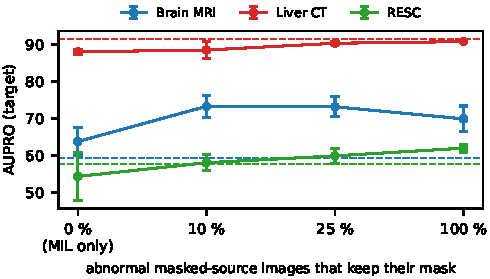
\includegraphics[width=\linewidth]{figures/fig1_budget.pdf}
  \caption{Label budget (round 3, mean $\pm$ SD over seeds 3--5): target AUPRO when masks are kept for 0, 10, 25 or 100\% of the abnormal masked-source images and MIL is used for all other images. Dashed: MVFA re-trained with full masks.}
  \label{fig:budget}
\end{figure}

\section{Experiments}
\label{sec:experiments}
\subsection{Image labels nearly match masks}
Table~\ref{tab:main} gives round 3. Without a single mask, MIL keeps 0.969 of MVFA's pixel-AUROC margin. Per target, this is 1.019 on brain MRI, 0.964 on liver CT and 0.924 on RESC, so it meets the pre-registered ``nearly matches'' grade ($\ge 0.90$ on every target). Only round 3 tested this under a frozen rule. Earlier rounds point the same way but are weaker: round 1 (0.966) used one seed and the released checkpoint as reference, and round 2 (0.930) fell to 0.716 on RESC. Against the released checkpoint R0, round 3 gives 0.916 (RESC 0.826). MIL's RESC spread is smaller than in round 2 (pixel SD 3.71 vs 9.90) but still the largest in Table~\ref{tab:main}. AUPRO shows the remaining gap: on liver CT, MIL reaches 88.08 against MVFA's 91.55, and in the four fixed examples of Fig.~\ref{fig:heatmaps} its maps look more diffuse.

\subsection{How many masks are needed?}
Masks help unevenly (Fig.~\ref{fig:budget}).
\begin{itemize}
\item \textbf{Liver CT:} AUPRO rises towards MVFA as masks are added, but no budget reaches it. With 10\% masks the mean pixel-AUROC difference from MVFA is $-1.96$, so the pre-registered ``10\% matches MVFA'' rule (no worse than $-1$ on every target) fails.
\item \textbf{Brain MRI and RESC:} every budget of 10\% or more is at or above MVFA.
\item \textbf{Full masks plus MIL:} adding MIL on the mask-less sources (MIL + 100\%) changes pixel AUROC by $+3.63$, $-0.88$ and $+2.74$, which meets the ``matches MVFA'' grade. Its AUPRO is higher than MVFA's in 6/9 pairs ($p=0.2539$), short of the ``beats MVFA'' grade.
\end{itemize}
The brain-MRI gain at 10\% was a post-hoc observation in round 3 (one of three budgets on three targets), so we tested it once more on fresh seeds 8--12 under a rule frozen in advance. MIL with 10\% masks beat MVFA in AUPRO on 5/5 seeds ($p=0.0312$): a mean gain of $+14.70$ AUPRO and $+5.35$ pixel AUROC (92.36 vs 87.00). This is one target and one test, and image AUROC did not improve ($+1.08$; MVFA's is noisy, $63.29\pm9.80$). The published MVFA reports 90.27 brain pixel AUROC with full data, 50 epochs and test-set selection; this crosses protocols, so we make no claim against it.

\begin{table}[t]
\centering
\scriptsize
\setlength{\tabcolsep}{2.5pt}
\begin{tabular}{@{}lll@{}}
\toprule
Claim tested (round) & Result & Outcome \\
\midrule
MIL keeps MVFA's localisation (3) & $\rho$ 0.969, min 0.924 & confirmed \\
10\% masks $>$ MVFA, brain (FU) & 5/5 seeds, $p=0.0312$ & confirmed \\
MIL + 100\% $>$ MVFA (3) & 6/9 pairs, $p=0.2539$ & matches \\
10\% masks match MVFA (3) & liver $-1.96$ pixel & trails \\
MIL $>$ MVFA, brain (2$\to$3) & 3/5 seeds, $p=0.5$ & not replicated \\
PU + 100\% $>$ MVFA (2$\to$3) & 5/9 pairs, $p=0.5$ & not replicated \\
Gated MIL $>$ MIL (2) & $-5.26/-1.15/+4.25$ & falsified \\
PU ($\pi=0.01$) $>$ MIL (2) & $-0.67/-4.01/-13.83$ & unsupported \\
PU fine-tune $>$ control (1) & 6/9 pairs, $p=0.2539$ & no gain \\
\bottomrule
\end{tabular}
\caption{Every pre-registered claim and its outcome, labelled as in the frozen rules (pixel-AUROC differences per target: brain / liver / RESC). Raw one-sided sign-test $p$; Holm-adjusted: 1.0 for both ``not replicated'' rows, 0.5078 for MIL + 100\%. Round 2 used 5 epochs and 3 seeds; the brain rows use seeds 3--7 (round 3) and 8--12 (FU: follow-up).}
\label{tab:record}
\end{table}

\begin{table}[t]
\centering
\scriptsize
\setlength{\tabcolsep}{4pt}
\begin{tabular}{@{}lcccc@{}}
\toprule
Image AUROC (round 3) & Brain & Liver & RESC & OCT17 \\
\midrule
MVFA re-trained (100\%) & 56.33 & 60.60 & 74.29 & 70.75 \\
MIL (0\%) & 67.50 & 67.95 & 71.27 & 62.13 \\
MIL + 10\% & 61.21 & 65.64 & 71.58 & 59.27 \\
MIL + 25\% & 58.62 & 68.05 & 72.71 & 64.63 \\
MIL + 100\% & 60.30 & 63.42 & 72.25 & 61.84 \\
PU + 100\% & 67.52 & 63.86 & 71.37 & 65.09 \\
\bottomrule
\end{tabular}
\caption{Target image AUROC (round 3, mean over seeds 3--5; OCT17 is scored by the RESC+OCT17 model). The published MVFA reports 78.63 / 76.24 / 83.31 on brain / liver / RESC under its own protocol.}
\label{tab:img}
\end{table}

\begin{figure*}[t]
  \centering
  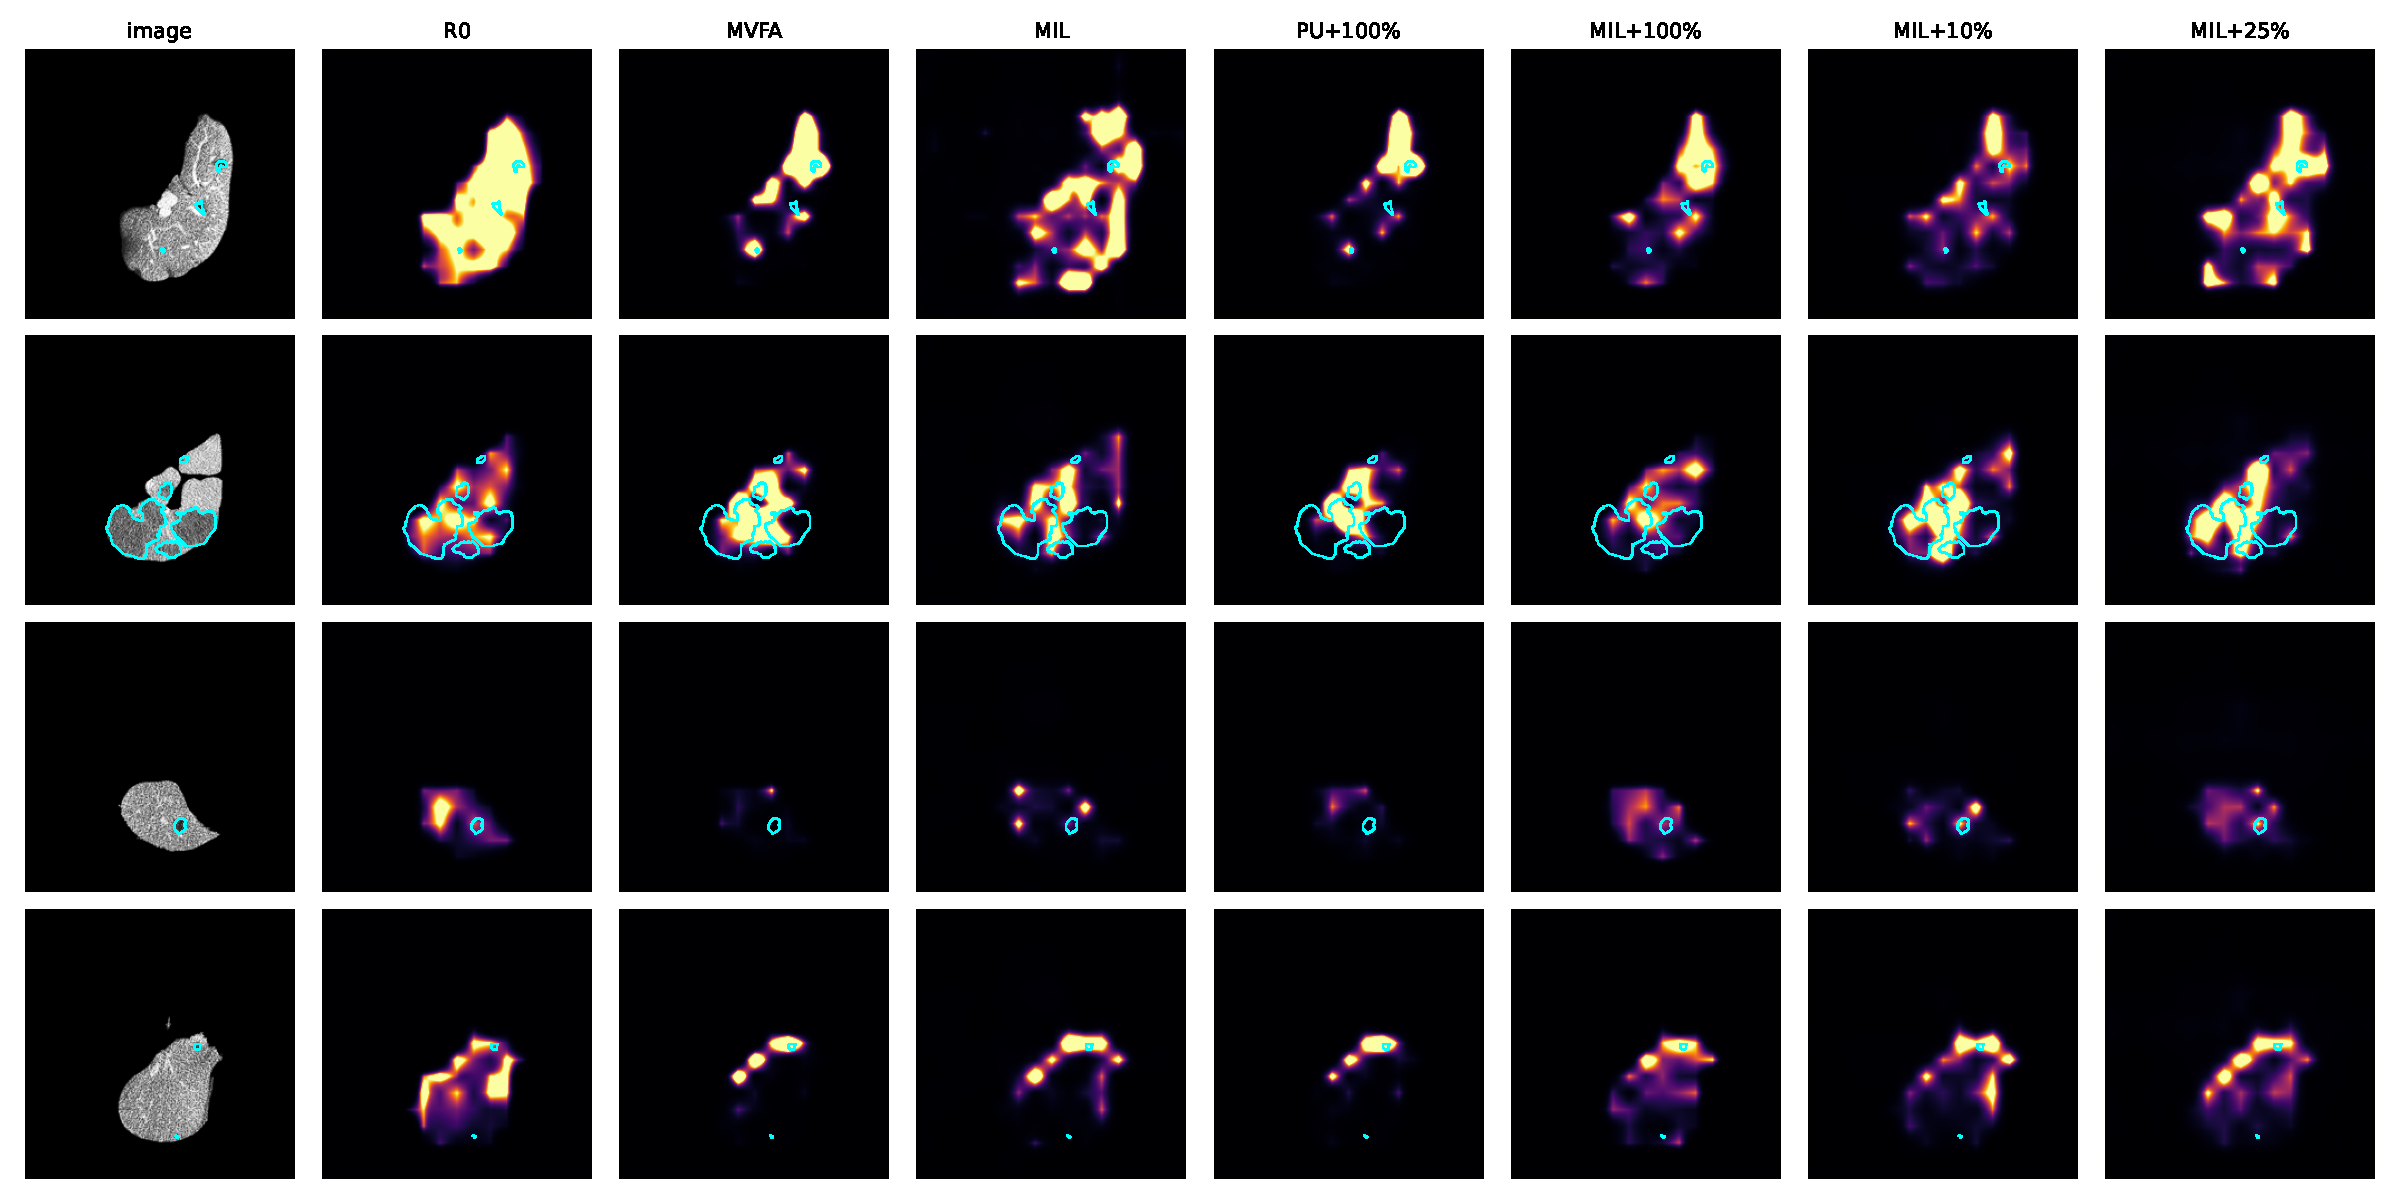
\includegraphics[width=0.85\textwidth]{figures/fig2_liver_heatmaps_r3.pdf}
  \caption{Liver CT heat maps (round 3, seed 3) for four test images fixed by a rule set before any map was viewed; cyan: ground-truth outline. Columns: image, R0, MVFA re-trained, MIL (no masks), PU + 100\%, MIL + 100\%, MIL + 10\%, MIL + 25\%. Illustrative only; liver CT is the target on which masks help most.}
  \label{fig:heatmaps}
\end{figure*}

\subsection{What did not hold}
Table~\ref{tab:record} lists every pre-registered claim.
\begin{itemize}
\item \textbf{Round 2's apparent wins did not survive.} Round 2 suggested that MIL beats MVFA on brain MRI and that PU + 100\% beats MVFA. Neither held after four times the training on fresh seeds: 3/5 and 5/9 pairs, both $p=0.5$.
\item \textbf{Gated MIL failed its rule.} Our rank-1 refinement selected lesion patches no more often than plain MIL (0.466 vs 0.493 of top-$k$ patches inside source masks), in a 3-seed, 5-epoch test.
\item \textbf{PU did not help in our setting.} Its class prior could not be estimated from MVFA's patch scores (round 1). With $\pi$ fixed at 0.01 it did not beat MIL (RESC $-13.83$), and a single-seed run at $\pi=0.05$ collapsed on liver (65.79). We did not tune $\pi$, so this tests our implementation, not PU learning in general.
\end{itemize}

\subsection{Analysis and limitations}
\begin{itemize}
\item \textbf{Where the top-$k$ patches land.} Masks mainly sharpen where the selected patches fall: the share inside source lesions (round 3, source validation images) rises from 0.452 (MIL) through 0.661 (10\% masks) to 0.787 (MVFA). Yet in the follow-up's brain fold, MVFA's 0.931 transfers worse than the 0.791 of 10\% masks. This is consistent with full masks over-fitting the source lesions' appearance, but it is a hypothesis we did not test.
\item \textbf{Reduced training budget.} We use a subsample and 20 epochs; MVFA uses full data and 50 epochs. Most runs peaked before their last epoch (11/58 chose it, against 37/57 in round 2), but 18/58 chose one of the last two, so longer training could still change the results.
\item \textbf{Weak image-level detection.} Target image AUROC is weak (Table~\ref{tab:img}) and fell with longer training: MVFA's brain image AUROC is 56.33 at 20 epochs, 65.73 at 5 epochs and 79.80 for the test-selected R0. We cannot separate the effect of source-only selection from that of the schedule. MIL is higher on brain and liver (67.5 and 67.95 vs 56.33 and 60.6) but lower on RESC and OCT17 (71.27 and 62.13 vs 74.29 and 70.75). Every re-trained arm stays below the published MVFA (78.63 on brain).
\item \textbf{Scope.} The study uses one base model and 3 seeds (5 for the two brain tests: seeds 3--7 and 8--12). RESC is held out together with OCT17, and chest X-ray was below chance (50) for every arm in round 2.
\item \textbf{Reproducibility.} The code, its tests, the frozen rules with their hashes, the split lists, every run's results and the run logs are kept with the paper. Trained adapters are archived separately.
\end{itemize}

\section{Conclusion}
\label{sec:conclusion}
For MVFA, localisation on an unseen medical modality does not require dense masks. Image labels alone keep about 97\% of the mask-supervised pixel-AUROC margin of a re-trained MVFA. A tenth of the masks plus image labels even improves localisation on brain MRI, though not on liver CT. The two refinements we implemented did not help, and pre-registered replication removed two apparent gains. Mask-efficient training should therefore start from plain MIL and be tested across seeds and schedules before any gain is claimed. Future work: test the 10\% budget on every target at MVFA's full schedule, check whether the effect holds for other CLIP-based detectors, and try mosaic MIL, which targets the lower lesion precision of MIL's patch selection.


\clearpage
{\small
\bibliographystyle{ieeenat_fullname}
\bibliography{references}
}
\end{document}
